\documentclass[12pt]{article}
\usepackage[margin=1.2in]{geometry}

\usepackage[utf8]{inputenc}
\usepackage{graphicx}
\usepackage{subcaption}
\usepackage{amsmath,amsthm,amssymb,enumitem,mathtools,titling}
\usepackage{multicol}
\usepackage{hyperref}
\usepackage[style=ieee,backend=bibtex]{biblatex} % citations
\usepackage{algorithm}
\usepackage{algpseudocode}

\graphicspath{ {../src/results} }

\newcommand{\lab}{\texttt{LAB}}
\newcommand{\slic}{\texttt{SLIC}}

\makeatletter
\newcommand{\StatexIndent}[1][3]{%
  \setlength\@tempdima{\algorithmicindent}%
  \Statex\hskip\dimexpr#1\@tempdima\relax}
\algdef{S}[WHILE]{WhileNoDo}[1]{\algorithmicwhile\ #1}%
\makeatother

\DeclarePairedDelimiterX\set[1]\lbrace\rbrace{\def\given{\;\delimsize\vert\;}#1}

\addbibresource{refs.bib}

\title{\vspace{-1cm} Segmentation par Superpixels}
\author{
  Tom Sarry \\
  \texttt{<tom.sarry@umontreal.ca>}
}
\date{D\'ecembre 2022}

\begin{document}

\maketitle

\section{Introduction}

La segmentation d'une image en plusieurs zones homog\`enes est un probl\`eme int\'eressant
et est utilis\'e dans de nombreux domaines en informatique comme l'imagerie m\'edicale ou encore la vision par ordinateur.
En effet, trouver de nombreuses zones uniformes permet de simplifier l'image, en regroupant les informations redondantes.

La m\'ethode utilis\'ee pour segmenter une image dont nous parlerons sera celle des \textit{Superpixels}:
zones homog\`enes et g\'eographiquement compactes.
Plusieurs algorithmes existaient en 2010 afin de segmenter une image de cette mani\`ere, mais poss\'edaient soit
trop de param\`etres, ce qui rendait leur utilisation complexe, ou ne fonctionnaient pas en temps lin\'eaire, propri\'et\'e cependant d\'esirable.

Nous pr\'esentons donc aujourd'hui l'algorithme \texttt{SLIC} \cite*{slic}, d\'evelopp\'e en 2010 par des chercheurs de l'EPFL,
fonctionnant en temps lin\'eaire en terme du nombre de pixels de l'image
et qui n'a pas besoin de param\`etres, \`a part le nombre de superpixels d\'esir\'es.
Cet algorithme de segmentation n\'ecessite moins de ressources que les autres options \`a disposition \`a l'\'epoque,
il \'etait donc adapt\'e pour des appareils moins puissants comme des petites cam\'eras ou des t\'el\'ephones.

\section{Algorithme}

L'algorithme \texttt{SLIC}, ou \textit{Simple Linear Iterative Clustering} s'effectue dans l'espace
de couleur \lab\ (L*a*b* CIE 1976\footnote{\url{https://fr.wikipedia.org/wiki/L*a*b*_CIE_1976}}),
afin de b\'en\'eficier de sa propri\'et\'e d'\^etre perceptuellement uniforme.
En effet, plusieurs couleurs paraissant \textit{aussi} diff\'erentes par le SVH (Syst\`eme Visuel Humain),
poss\`ederont une distance par norme $L_2$ similaire.

Cet algorithme utilise donc un espace de dimension 5: chaque pixel est assign\'e le 5-tuple suivant: $\langle x, y, l, a, b \rangle$,
qui correspond \`a sa position $\langle i, j\rangle$ dans l'image, ainsi que ses param\`etres de couleurs.
Cela nous permet donc de calculer une distance pixel \`a pixel qui prend en compte l'\'eloignement physique,
mais aussi l'importance de la differ\'erence de couleurs entre ceux-ci.

La proc\'edure est tr\`es similaire \`a l'algorithme \textit{K-means} et se d\'eroule de la mani\`ere suivante, un pseudocode simplifi\'e est \'egalement donn\'e dans l'Algorithme \ref{alg:slic}:

\begin{enumerate}
  \item \textbf{Initialisation des Centres:} Les $k$ centres pour les superpixels sont plac\'es \`a interval regulier pour quadriller l'image initiale.
  \item \textbf{Ajustement des Centres:} Les centres ont possiblement \'et\'e positionn\'es sur des pixels \`a fort gradient, ie. sur un contour.
        Il est pr\'ef\'erable si c'est le cas de bouger l\'eg\`erement le centre en choissant le pixel \`a plus faible gradient dans son voisinage $3\times 3$.
  \item \textbf{R\'ep\'eter jusqu'\`a convergence ($E \leq 1$):}
        \begin{enumerate}
          \item \textbf{Assignement des R\'egions:} Pour chaque pixel, calculer la distance entre celui-ci et tous les centres pr\'esents dans son voisinage restreint\footnote{Un carr\'e de $2S$ pixels de c\^ot\'es, o\`u si $N$ est le nombre de pixels de l'image, $S=\sqrt{\frac{N}{k}}$}.
                Cette distance entre deux pixels $s$ et $t$ se fait dans un espace de dimension 5 et se calcule de la mani\`ere suivante:
                \begin{align*}
                  D_{s,t} = \sqrt{(x_s - x_t)^2 + (y_s - y_t)^2 + (l_s - l_t)^2 + (a_s - a_t)^2 +  (b_s - b_t)^2}
                \end{align*}
                Par la suite, on assigne la region de ce pixel comme \'etant la region du centre avec lequel il avait la plus petit distance,
                ie. le plus de similarit\'es.
          \item \textbf{Mise \`a jour des Centres:} Pour chaque centre, mettre \`a jour ses valeurs $\langle x, y, l, a, b\rangle$,
                en prennant la moyenne des valeurs des pixels contenus dans sa r\'egion.
          \item \textbf{Calcul de la Convergence:} Calculer $E$: la norme $L_1$ entre les pr\'ec\'edents centres et ceux venant d'\^etre calcul\'es.
        \end{enumerate}
  \item \textbf{Garantir la Connectivit\'e:} Apr\`es avoir atteint convergence, il est possible qu'une r\'egion soit disjointe.
        Nous englobons donc les parties de r\'egion qui n'appartiennent pas \`a la zone \textit{principale} de la r\'egion (celle qui inclue le centre de la r\'egion),
        par la r\'egion la plus importante qui jouxte cette zone disjointe.
\end{enumerate}

\begin{algorithm}
  \caption{\slic}
  \label{alg:slic}
  \begin{algorithmic}[1]

    \Procedure{slic}{$nSuperpixels$}

    \State Initialize $nSuperpixels$ centers on a grid at regular interval
    \State Move centers to the lowest gradient in their $3 \times 3$ neighborhood

    \Repeat

    \ForAll{cluster centers}
    \State Assign neighboring pixels to this cluster if this center has the lowest
    \StatexIndent[3] \texttt{xylab}-distance to them
    \EndFor

    \State Compute new cluster centers by taking the average of the $\langle x, y, l, a, b \rangle$ values
    \StatexIndent[2] in each cluster
    \State $E \gets L_1$ distance between old and new cluster centers
    \Until{$E \leq$ threshold} \Comment{$E \leq 1$ in the code}

    \State Enforce connectivity

    \EndProcedure

  \end{algorithmic}
\end{algorithm}

\section{R\'esultats}

Nous pr\'esentons dans cette section les r\'esultats obtenus par l'algorithme sur deux image \texttt{Church} et \texttt{Lady} utilis\'es dans le papier original, cf Figure \ref{fig:church_segm} et \ref{fig:lady_segm}.

\begin{figure}
  \begin{subfigure}{0.49\textwidth}
    \centering
    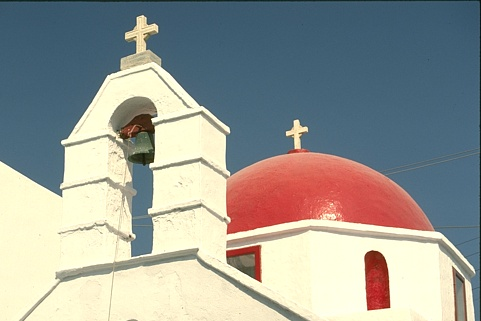
\includegraphics[width=1\textwidth]{church/church.png}
    \caption{Image originale}
  \end{subfigure}
  \begin{subfigure}{0.49\textwidth}
    \centering
    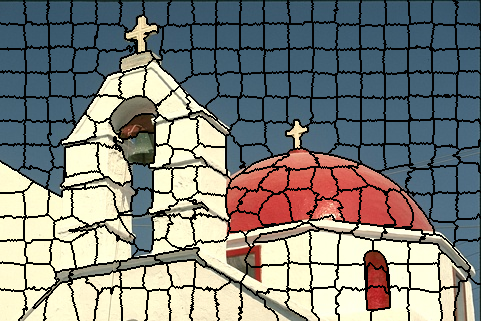
\includegraphics[width=1\textwidth]{church/church_segmented_256.png}
    \caption{$n=256$}
  \end{subfigure} \\
  \begin{subfigure}{0.49\textwidth}
    \centering
    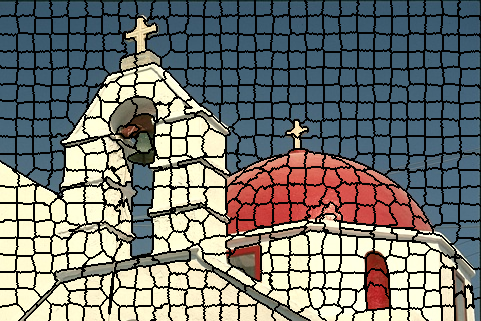
\includegraphics[width=1\textwidth]{church/church_segmented_512.png}
    \caption{$n=512$}
  \end{subfigure}
  \begin{subfigure}{0.49\textwidth}
    \centering
    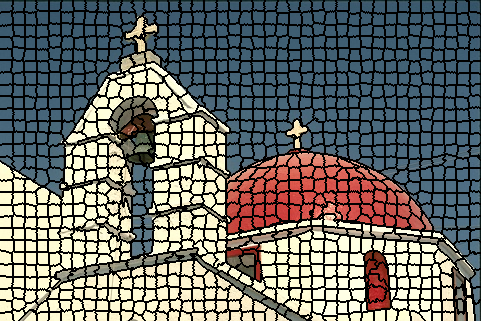
\includegraphics[width=1\textwidth]{church/church_segmented_1024.png}
    \caption{$n=1024$}
  \end{subfigure}
  \caption{Image originale et segment\'ee de l'image \texttt{Church}.}
  \label{fig:church_segm}
\end{figure}

\begin{figure}
  \begin{subfigure}{0.48\textwidth}
    \centering
    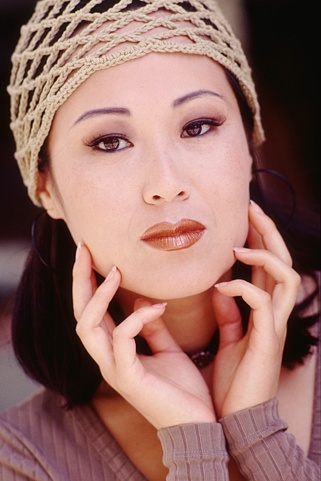
\includegraphics[width=0.8\textwidth]{lady/lady.png}
    \caption{Image originale}
  \end{subfigure}
  \begin{subfigure}{0.48\textwidth}
    \centering
    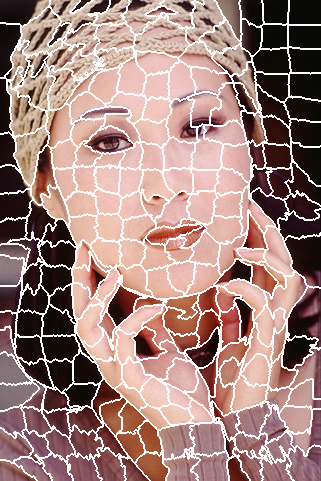
\includegraphics[width=.8\textwidth]{lady/lady_segmented_256.png}
    \caption{$n=256$}
  \end{subfigure} \\
  \begin{subfigure}{0.48\textwidth}
    \centering
    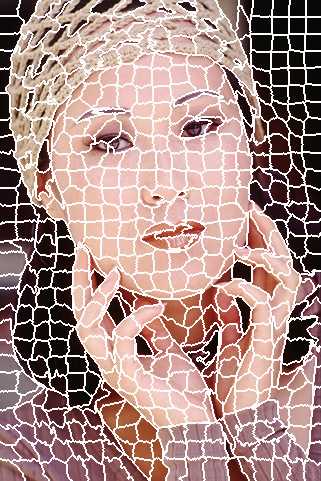
\includegraphics[width=.8\textwidth]{lady/lady_segmented_512.png}
    \caption{$n=512$}
  \end{subfigure}
  \begin{subfigure}{0.48\textwidth}
    \centering
    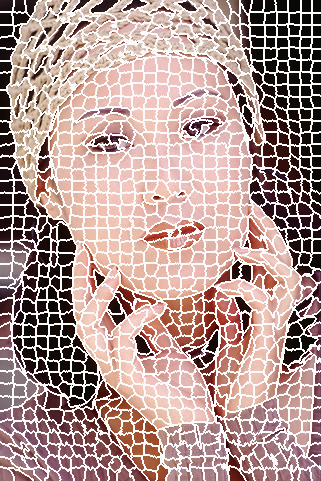
\includegraphics[width=.8\textwidth]{lady/lady_segmented_1024.png}
    \caption{$n=1024$}
  \end{subfigure}
  \caption{Image originale et segment\'ee de l'image \texttt{Lady}.}
  \label{fig:lady_segm}
\end{figure}

\section{Discussion}

\section{Conclusion}

\AtNextBibliography{\small}
\printbibliography


\end{document}